\documentclass[12pt]{amsart}	
\usepackage{amssymb}
\usepackage{amsthm}
\usepackage{mycros}
\usepackage[margin=1in]{geometry}
\usepackage{graphicx}
\setlength{\parskip}{1em}
\setlength{\parindent}{0em}
\newtheorem{theorem}{Theorem}

\def\al#1{\begin{align*} #1 \end{align*}}
\def\Nrd{{\rm Nrd}}
\def\Trd{{\rm Trd}}
\def\Nm#1{{\rm Nm}_{#1}}

\newcommand{\vpi}{\varpi}
\newcommand{\subsetc}{\underset{\text{conj}}{\subset}}
\newcommand{\Scc}{[S]}

% \newtheorem{definition}{Definition}
% \title{Trace determined subgroups}
% \author{Justin Katz}
\begin{document}

%\maketitle

% %!TEX root = main.tex
\begin{theorem}
	$\Gamma_0(\pfrak^n)$ is trace maximal.
\end{theorem}

 
% %!TEX root = main.tex
\begin{figure}
	\centering
	\scalebox{.5}{
	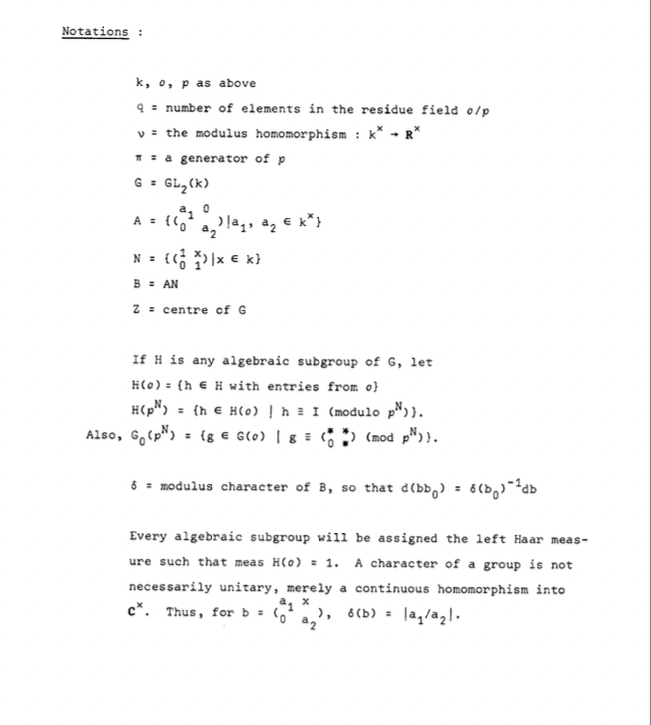
\includegraphics{
	branch-decompositions-notation.png}
	}
\end{figure}

An admissible rep of $G$ is complex vector space $V$ and a $\rho : G \to \Aut(V)$ such that 
\begin{itemize}
	\item For all $v\in V$, the stabilizer of $v$ in $G$ is an open subgroup; this is needed for matrix coefficients of $V$ to be \emph{locally constant}. This is smoothness
	\item For each compact open subgroup $K\leq G,$ the $K$-fixed vectors $V^K$ form a finite dimensional subspace.
\end{itemize}

For a character $\mu :A \to \C^\times$, extend $\mu$ to $B=NA$ so that $\mu(n) =1$ for all $n\in N$, and define the space of $\Ind(\mu)$ to be the space of locally constant functions $f: G \to \C$ such that $f(n a g) = \delta^{1/2}(n a)\mu(n a)f(g)$. 



% For a group $G$ and a subgroup $H\leq G$, let $\pi : G \epi G/H$ be the canonical projection. Then $G$ is a principal $H$ bundle over $G/H$; this is tautological.

% Let $s: G/H \to G$ be a section (supposing one exists in the relevent category).  

% Given a representation $\rho$ of $H$ on a space $V$. The associated bundle is $G\times V \rmod (g,v) \sim (gh, \rho(h^\inv ) v) := G \times_H V \epi G/H$    via $\pi(g,v) = g H$. I.e.: sitting above each point $gH \in G/H$ is a copy of $V$.  

\def\Map{\rm Map}
% Let 
% \[
% \Map_H(G,V) = \{ f: G \to V \vert f(gh) = \rho(h^\inv) f(g)\, , (g,h) \in G\times H \}.
% \]

% This space of $V$ valued functions on $G$ can be identified with the space $\Gamma(E_V)=\Gamma(G,H,V)$ of sections $s: G/H \to E_V = G\times_H V$. Explicitly, given $f\in \Map_H(G,V)$, define a section $s$ by $s(gH)=(g,f(g)).$

In the description of $\Ind_B^G(\mu)$ as a space of functions on $G$ which are $(B,\mu)$  equivariant, view all of the $\Ind_B^G(\mu)$ as living inside some suitably large space of complex valued functions on $G$. One can do this in such a way that there is a consistent action of $G$ on functions \emph{by translation}. Other models substitute, for example, a consistent action for a consistent underlying space of functions. 

Keeping notation consistent with Bill's, $PS(\mu)$ is the principal series, and is associated to a $\mu : A \to \C^\times$. 

The definition of admissibility is designed so that the contragredient representation $\tilde{\rho}$ of admissible $\rho$ is admissible. The underlying space of $\tilde{\rho}$ is the collection of linear functionals on $\rho$ which are fixed by some open subgroup of $G$.

Integration yields a hermitian pairing $PS(\mu)\times PS(\mu^\inv ) \to \C$, so that $PS(\mu^\inv)$ is the contragredient to $PS(\mu)$. The underlying mechanism is that there is a unique $G$ invariant linear functional $I$ on $\Ind(\delta^{1/2})$ such that on the subspace of smooth compactly supported function $f: G \to \C$, one has $I(P_\delta f(g)) = \int_G f(g) \dop g$, where $P_\delta f(g) = \int _B f(bg) \dop b. $

Given an admissible representation $\rho$ of $G$ on a space $V$, set 
\[
	V(N) = \{ v  :  \int_\bfrak \rho(\tbt{1}{x}{0}{1} ) v \dop x = 0  \text{ some fractional ideal } \bfrak \}.
\]


% \subsection{Some comments on choices}
% Briefly lets let $\kfrak$ be algebraically closed, and $G=\GL(V)$ where $V$ is a two dimensional vectorspace over $\kfrak$

% Picking a maximal torus $T$ in $G$ amounts to picking a pair of linearly independent lines in $V.$ Note, this is not quite the same as picking a basis. These lines are the common eigenspaces of every element of $T$. 

% Picking (one of the two possible) orderings on the two roots of $T$ in $G$ amounts to a choice of borel $B$ containing $T$.  
\def\Aff{\rm Aff}
\section{Cartan Decomposition}
Let $G$ act on the set of ordered bases of $\kfrak^2$ by letting $g=\tbt{a}{b}{c}{d}$ send $(e_1,e_2)$ to $(ae_1 +b e_2 , ce_1 +de_2).$ 

Given an ordered basis $(e_1,e_2)$, let $\langle e_1,e_2\rangle = \ofrak e_1 + \ofrak e_2  \leq \kfrak^2$ be the lattice generated by it. 

Let $L=\langle u_1,u_2 \rangle $ be the lattice generated by the standard basis and $L'= gL$ the lattice generated by $g(u_1,u_2).$

Elementary divisor theorem implies there exists an $\ofrak$ basis $(v_1,v_2)$ of $L$ and elements $a_1,a_2 \in \kfrak^\times $ with $a_1 \in \ofrak a_2$ such that $(a_1v_1,a_2v_2)$ is a basis for $L'$. 

That is, there exists a $k_1 \in \GL_2(\ofrak)$ sending $(u_1,u_2)$ to $(v_1,v_2)$, and another $k_2 \in \GL_2(\ofrak)$ such that $k_2 g(u_1,u_2) = (a_1 v_1, a_2 v_2).$ If $a = \tbt{a_1}{}{}{a_2}$ then $k_2 g = a k_1$.  

Leting $A^{-}  = \{\tbt{a_1}{}{}{a_2}: \, a_1 \in a_2 \ofrak \}$, we have shown
\[ \boxed{
\GL_2(\kfrak) = \GL_2(\ofrak) \cdot A^{-} \cdot \GL_2(\ofrak), 
}\]

\section{Iwasawa decomposition} 
$\GL_2(\kfrak)$ acts transitively on $\Pbb^1(\kfrak)$. The stabilizer of any point is conjugate to the standard borel $B(\kfrak)$ of upper triangulars (equivalently, any point in $\Pbb^1$ can be taken to $\infty$).

Restricting the surjection $G(\kfrak) \to G(\kfrak) / B(\kfrak) = \Pbb^1(\kfrak)$ to $G(\ofrak)$ remains surjective, and induces an identification of $G(\ofrak) / B(\ofrak)$ with $\Pbb^1(\kfrak)$. 

\section{Iwahori factorization}
Every element $g \in G_o(\pfrak)$ has a unique decomposition $n^{-} b$ with $n^{-} \in N^{-}(\pfrak)$ and $b\in B(\ofrak)$:
\[ 
	\boxed{
		G_o(\pfrak) = N^{-} (\pfrak) B(\ofrak). 
	}
\]

Indeed, if $c\in \pfrak$ then $a \in \ofrak^\times$  and 
\[ \Tbt{a}{b}{c}{d} = \Tbt{1}{0}{c/a}{1} \cdot   \Tbt{a}{b}{0}{d-bc/a} \]
% %!TEX root = main.tex

Given a group $G$, a field $k$, and a class function $\tau : G \to k$, say that a subgroup $H\leq G$ with $\tau(H) = S$ is $(S,\tau)$-maximal if for all $H < K \leq G$ with $\tau(H) = \tau(K)$, one has $H = K$. Let $X(S, \tau, G) $ be the collection of $(S, \tau)$ maximal subgroups of $G$.

Let $\Inn:G \to \Aut(G)$ denote the conjugation action $\Inn(g)x = g x g^\inv,$ at both the level of elements and subgroups. Then $X(S, \tau, G)$ is $\Inn(G)$ stable. 

Say that $S\subset k$ is $(\tau, G)$ if $\Inn(G)$ acts transitively on $X(S, \tau, G)$. 

%%%%%%%%%%%%%%%%%%%%%%%%%%%%%%%%%%%%%%%%%%%%%%%%%%%%%%%%%%%%%%%%%%%%%%
\section{The metatheorem}
%%%%%%%%%%%%%%%%%%%%%%%%%%%%%%%%%%%%%%%%%%%%%%%%%%%%%%%%%%%%%%%%%%%%%%

Let $B$ be an indefinite quaternion algebra over a number field $K$, satisfying condition  (*)\footnote{$K$ should be  a totally real field, with odd class number, and $B$ should be a split over a unique real place of $K$}. 

Let $\Nrd: B\to K$, and $\Trd: B \to K$ denote the reduced norm and trace maps respectively. The canonical involution $\bar{\cdot}$ on $B$ satisfies $x\bar{x} = \Nrd(x) 1 \in K$ and  $x+\bar{x} = \Trd(X) 1 \in K$, where we identify in both cases $K$ with the center of $B$. 

Further, suppose that $B$ has type number $1$, so that $B$ has a unique $B^\times$ conjugacy class of maximal orders. Pick one, say $\Ofrak$. 


% \begin{itemize}
% 		 	\item $p$ in $P < \Ocal < K$, $\pi$ in $\Pcal$;
% 		  	\item $q_n : \Ocal \to Q_n = \Ocal / \Pcal^n$, $q  = q_n, k = Q_1$;
% 		  	\item Pick a section $\xi_n : Q_n \to \Ocal $compatible with transition map
% 		  	\item $G$ semisimple rank 1 over $K$; $\gfrak$ its lie algebra
% 		  	\item $r_n : G(\Ocal) \to G(Q_n)$ induced by map on $\Ocal$;
% 		  		\begin{itemize}
% 		  			\item $A$ is the maximally split torus in $G$. As an algebraic group is $\Gbb_m$, since rank 1. 
% 		  			\item Pick a root $\alpha: A \to \Gbb_m $, and designate it positive, let $u=u_\alpha: \Gbb_a \to G$ be a parameterization of the associated unipotent $U=U_\alpha$; 
% 		  			\item $B$ is the associated borel, with unipotent radical $U$, and factorization $B=AU$ semidirect, with $\Ad(a)u(x)= u(\alpha(a) x)$ for $a \in A$ and $x\in \Gbb_a$. The opposite unipotent is $\Ubar=U_{-\alpha}$, one which $A$ acts by the character $\alpha^\inv$. 
% 		  			\item The sequence $\Gbb_a \xrightarrow{u_\alpha} B \to B/U$ exhibits $B$ as a line bundle over $B/U$. The cocharacter $\check{\alpha}: \Gbb_m \to A \leq B \leq G$ yields a section: $\check{\alpha} \times u : \Gbb_m \times \Gbb_a \to B$ are global coordinates on this (apparently trivial) bundle. 
% 		  			\item $A$ acts on the fibers of $B \xrightarrow{\alpha} A$. In $u$ coordinates:
% 						\al{
% 						a\cdot u(x)\cdot a' \cdot u(y) 
% 						&= a \cdot \Ad(a')u(x) \cdot  u(y) \\
% 						&=  a \cdot u(a'^\alpha  u) \cdot u(y) \\
% 						&= a \cdot u(  a'^\alpha  x + y )
% 							}
% 					\al{ 
% 						u(x)\cdot a\cdot u(y) 
% 						&= \Ad(a) u(a^{-\alpha} x) \cdot a \cdot u(y) \\
% 				   		&= a \cdot u(a^{-\alpha} x )\cdot u(y) \\
% 				   		&= a \cdot u(a^{-\alpha} x +y)
% 				   			}
% 	  				shows that the action of $U= \Gbb_a$ on the line affine line $\Abb^1 = \{a\} \times U$ over $a \in A$ in $B$ is 
% \[  x \times y \mapsto a^{- \alpha} x + y \]
% 		  		\end{itemize}
% 		  	\item $\rho_n : G(Q_n) \to G(\Ocal)$ a section of $r_n$; 
% 		  	\item $\tau : G(K; \Ocal; Q_n) \to K; \Ocal; Q_n$, natural and $\Inn(G) (K; \Ocal; Q_n)$ invariant 
% 				% \subitem Open subsets of $K$ of form $ q_n^\inv (S)$ for a (finite) subset $S$ subset $Q^n$. It is of the form $\cup_{s in S} q_n^\inv(s) s  = \cup_{s in S} (\sig_n(s) + \Pcal^n)$
% 				% \subitem Open subsets of $G(K)$ 
% \end{itemize} 

% For $S \subset G$, write $S^G = \cup_{s \in S} s^G = \cup_{s\in S, g\in G} \{ s^g\}$. 

% %!TEX root = main.tex

For $\tbt{a}{b}{c}{d} \in G = \SL(2,k)$, if $c \in k^\times$ then one has 
\al{ 
    \Tbt{a}{b}{c}{d} &= \Tbt{-1}{}{}{-1}  \Tbt{c^\inv}{}{}{c} \Tbt{1}{ac}{}{1} \Tbt{}{1}{-1}{} \Tbt {1}{dc^\inv}{}{1} \\
    				 &= \abf (-1)\cdot \abf (c^\inv)\cdot \ubf (ac) \cdot \wbf \cdot \ubf(dc^\inv)
}
while if $c=0$, then $d=a^\inv$
\al{
	\Tbt{a}{b}{0}{a^\inv} &= \Tbt{a}{}{}{a^\inv} \Tbt{1}{ba^\inv}{}{1} \\
						  &= \abf(a)\ubf(ba^\inv) 
}
Here, $\abf: \Gbb_m \to G$ is the cocharacter corresponding to the split maximal torus $A \leq G$, $\ubf: \Gbb_a \to G$ parameterizes the associated root subgroup, and $\wbf = \tbt{}{1}{-1}{}$ is the weyl element.

For $b \in k^\times$, one has 
\al{
	\abf(b) &= w \cdot \ubf(b^\inv)\cdot w\cdot \ubf (b) \cdot w \cdot \ubf(b^\inv)
			}


Some computations for posterity: 
\al{
	w*g*w &= \left(\begin{array}{rr}
-d & c \\
b & -a
\end{array}\right) \\
	w*g	  &= \left(\begin{array}{rr}
c & d \\
-a & -b
\end{array}\right) \\
	g*w   &= \left(\begin{array}{rr}
-b & a \\
-d & c
\end{array}\right)
}

% %!TEX root = main.tex
Sally and Shalika notation:
\begin{itemize}
	\item $k$ is a local field, $\Ocal$ its ring of integers, $\pfrak$ its maximal ideal, $q= \|\Ocal /\pfrak \|$ is assumed odd. 
	\item Normalize the haar measure $\dop x$ on $(k,+)$ so that $ \Ocal$ has measure $1$. 
	\item Define the valuation on $k$ via the equations $\dop (ax)= \|a\| \dop x$ for $a\in k$. Let $U= \{x\in k : \|x\|=1\} = \Ocal^\times$ and $U_n = 1 + \pfrak^n = \{x \in U : \|x-1\| \leq q^{-n}\}$
	\item $\tau$ denotes a fixed uniformizer of $\pfrak$, $\eps$ is a fixed generator for the $q-1$th roots of $1$ in $U$. 
\end{itemize}

For $V$ a quadratic extension of $k$, we let $\Nm{V/k}$ denote the norm map. Since $k$ has odd residual characteristic, $V$ is one of $k(\sqrt{\tau}),$ $k(\sqrt{\eps \tau}),$ or $k(\sqrt{\eps})$. The former two are ramified, and the latter is unramified. We will use $\theta$ to represent one of $\tau, \eps \tau,$ or $\eps$.  

\def\cond#1{{\rm cond}(#1)}
For $V=V_\theta = k(\sqrt{\theta})$, we let $C_\theta = \ker \Nm{V/k} \leq V^\times$ and $\pfrak_\theta$ the prime ideal in $V_\theta$. Set, in the unramified case, for $h\geq 1$:
	\[ C_\eps ^{h} = (1 +\pfrak_\eps ^h) \cap C_\eps \] 
and in either of the ramified cases, for $h\geq 0$:
	\[ C_\theta^h  = (1+\pfrak_\theta^{2h+1})\cap C_\theta.\]

Then, in any case, $\{ C_\theta ^h \}$ constitute a neighborhood base about $1$ in $C_\theta$. For a character $\psi \in \hat{C_\theta}$, write $\cond{\psi}$ for the largest subgroup in this filtration on which $\psi$ is trivial. For each $\theta,$ $C_\theta$ has a unique character of order $2$ which we denote by $\psi_o=\psi_{o,\theta}$. 

Let $G = \SL(2,k),$ $A=A(k)$ the diagonal subgroup (a maximal split torus). This subgroup is isomorphic to $k^\times$. We let $A_d$ denote the image of $U_d$ under this identification. 

Let $T$ be any compact cartan in $G$, which must be naturally isomorphic to some $C_\theta$. Let $T_d$ denote the image of $C_\theta ^d$ under such an identification. 

For a subset $S$ of $G$, let $S^G = \{ g s g^\inv : g \in G, s \in S\}$, and let $S'$ the subset of $S$ consisting of regular elements (those with distinct eigenvalues). 
%%%%%%%%%%%%%%%%%%%%%%%%%%%%%%%%%%%%%%%%%%%%%%%%%%%%%%%%%%%%%%%%%%%%%%%%%%
\section{From SS paper on fourier transforms}
For $f \in C_c^\infty(G)$, define, for $\gamma$ noncentral, the orbital integral 
	\[I_f (\gamma) = \int _{G/G_\gamma} f(x \gamma x^\inv) \dop \xdot \]
where $G_\gamma$ is the centralizer of $\gamma$ in $G=\SL(2,k)$ and $\dop \xdot$ is a $G$ invariant measure on $G/G_\gamma$. 

We can view the map $f\mapsto I_{f}$ as one from $C_c^\infty (G)$ to $C(G)^{\Inn(G)}$, i.e. sending functions on $G$ to class functions. The naive quotient of $G$ by $\Inn(G)$ is a singular space (owing to the non-regular elements, as well as the unipotent elements) 

\begin{align*}
	A &= \{ \Tbt{\lambda}{}{}{\lambda^\inv} : \lambda \in k^\times \}, & 	&	  \\
	T_\tau &= \{\Tbt{x}{y}{\tau y}{x} : x,y \in k\},  & T^\# _\tau &= \{\Tbt{x}{\eps y}{\tau \eps^\inv y}{x} : x,y \in k\} \\
	T_{\eps \tau} &= \{\Tbt{x}{y}{ \eps \tau y}{x} : x,y \in k\}, & T^\# _{\eps \tau} &= \{\Tbt{x}{\eps y}{\tau y}{x} : x,y \in k\}\\
	T_{\eps} &= \{\Tbt{x}{y}{ \eps y}{x} : x,y \in k\},  & T^\# _{\eps} &= \{\Tbt{x}{\tau y}{\eps \tau^\inv y}{x} : x,y \in k\}
\end{align*}

When $-1 \in (k^\times)^2$, these constitute a complete (and irredundant) set of conjugacy classes of cartans in $G$. 

When $-1 \notin (k^\times) ^2$, $T_\theta$ and $T_\theta^\#$ are conjugate for $\theta \in \{ \tau, \eps \tau\}$. 

The set of elliptic elements in $G$ is 
\[
	G_e = \bigcup_{T'} (T')^G,
\]
as $T'$ runs through the collection $\{ T_\theta, T^\#_\theta : \theta \in \{\tau,\eps \tau, \eps \}\}$ of compact cartans in $G$. 

%!TEX root = main.tex

% Stealing some notation from Sally and Shalika: $k$ is the local field, with integers $\Ocal$, and $G=\SL_2(k)$. We let $K_m \leq \SL_2(k)$ be the kernel of the reduction mod $\Pcal^m$ map. $A$ is the diagonal split torus. 

%From Labesse and Langlands:


$F$ is a local field of characteristic zero, $G=\SL(2)$. Take a cartan subgroup $T$ of $G$, defined over $F$.  A special role will be played by the group $H^1(F,T)$. 

Set $\tilde{G}=\GL_2$, then $\Tilde{T} = C_{\tilde{G}} (T)$ is a cartan subgroup of $\tilde{G}$. That $\tilde{G}$ has a single $\tilde{G}(F)$ conjugacy class of cartans, one has $H^1(F,\tilde{T}) = 1.$  

Any $h\in \tilde{G}(F)=\GL(2,F)$ is a product $s^\inv g$ with $g\in G(\Fbar)=\SL(2,\Fbar)$ and $s \in \tilde{T}(\Fbar)$.

Let $L$ be the centralizer of $T(F)$ in the algebra of $2\times 2$ matrices over $F$. Then the \emph{set} of determinants of elements in $\tilde{T}(F)$ coincides with the algebra-theoretic norms of elements in $L^\times$.

The map $g \to \det h \mod \Nm{L/F} L^\times$ yields an identification of $F^\times / \Nm{L/F}$ with $H^1(F,T)$. 

If $F$ is an extension of a field $E$, consider groups $G'$ defined over $E$ sandwhiched between the restrictions of scalars: $\Res_{L/E}G \leq G' \leq \Res_{L/E}\tilde{G}$. Then $G'$ is defined by a subgfroup $A$ of $\Res_{L/E} \Gbb_m$ and $G'(F) = \{ g \in \tilde{G}(F) \vert \det g \in A (E)\}$

Take $T' = C_{G'}(\Res_{F/E}T)$ and set $\Dfrak(T';E) = F^\times / A(E)\Nm{L/F}L^\times $. A slight extension is to consider $G' = \{ g \in \tilde{G} (F) \det g \in A\}$ for any closed subgroup $A$ of $F^\times$, which may or may not be the set of points of a group rational over some field. 

Let $\kappa : X_* (T) \to \C^\times $ which is $\Gal(\Fbar)$ invariant. 

The LLC associates to the pair $(T,\kappa)$ a group $H$, which must be either $G$ or $T$. 

Fix haar measures on $G'$ and $T'$ and let $\gamma \in T'$ be regular. For $ h \in \tilde{G}(F)=\GL (2,F) $, we can transfer the measure on $T'$ to $h^\inv T' h $. 

Def: $G'$ over $F$ is an inner twist if there exists an isomorphism $\psi: G' \to G$ defined over an extension $K/F$ such that $\sigma(\psi) \sigma ^\inv$ is inner for all $\sigma \in \Gal(K/F).$ Langlands' prediction is that there should be an injection of the automorphic representation of $G'(\Abb_F)$ into those of $G(\Abb_F)$


Consider $\gamma' \in G'(F)$, semi-simple, then the conjugacy class of $\psi(\gamma')$ is defined\footnote{what does this mean here? I think this means that the conjugacy class of $\psi(\gamma')$ is stable under $\Gal(K/F)$, perhaps pointwise so}  over $F$. Steinberg assures us that the conjugacy class of $\psi(\gamma')$ in $G(\Fbar)$ contains an element $\gamma \in G(F)$. This means that there is an injection of the elliptic (i.e. nonsplit) conjugacy classes of $G'(F)$ into those of $G(F)$. These classes form the indexing set for the respective trace formula for $G'$ and $G$. One wonders if this injection respects the orbital integrals in some sense. 

For $\gamma \in T$ let $\gamma_1,\gamma_2 \in \bar{F}$ be its eigenvalues. When $T$ is split, the function $d(\gamma)= \frac{|(\gamma_1 -\gamma_2)^2|^{1/2}}{|\gamma_1\gamma_2|^{1/2}} $ will play a special role. 

Fix a regular element $\gamma^0$ in $\Tti(F))$ and let $\psi$ be a fixed nontrivial additive character of $F$. Fix an ordering $\gamma_1^0, \gamma_2^0$ on the eigenvalues of $\gamma^0$, which in turn determines an order on those for $\gamma$. 

For a given regular $\gamma$, the quotient $\Tti(F) \lmod \Gti(F)$ may be identified with the orbit $\Ocal(\gamma)$ of $\gamma$ under $\Gti(F)$ conjugation.

We arrange for the measure on $\Tti(F)\lmod \Gti))$ is of the ofrm $|\omega_\gamma |/|\gamma_1 - \gamma_2|$ for a certain form $\omega_\gamma$.

For $a\in F^\times$, set $\gamma(a) = a\tbt{1}{1}{0}{1}$. If $\Tti$ is split and $a\in Z(T'),$ set $\Phi^{T'}(a,f)= |a|^\inv \int_{\Ocal(\gamma(a))} f(h) \dop h$. 

For a quadratic extension $L/F$, regard $\Gti(F)$ as the group of invertible $F$ linear transformations of  $L$. Then $\Tti(F)= L^\times$ acting on $L$ by multiplication. 

Pick an $F$ basis $\{1,\tau\}$ for $L$. Then there are $u,v \in F$ so that $\tau^2 = u \tau +v$. 

If $\gamma = a+b\tau \in \Tti(F)$ or $L^\times$, its eigenvalues are of the form $\gamma_1=a+b\tau$ and $\gamma_2 = a+b \bar{\tau}$ so that $\gamma_1-\gamma_2  = b (\tau -\bar{\tau})$. 

In these coordinates, $\gamma$ corresponds to $\tbt{a}{bv}{b}{a+bu} $

For $g = \tbt{a_1}{b_1}{c_1}{d_1}$, then 
$$\gamma^g = \tbt{*}{-b \Nm{L/F}(b_1+d_1v)/\det g}{b \Nm{L/F}(a_1+c_1v)/\det g}{*}$$

Let $\Gti(\Ocal_F)$ be the stabilizer of $\Ocal_L$ in $\Gti(F)$. After averaging a function $f$ on $\Gti(F)$ over $\Gti(\Ocal_F),$ we can assume that $f(g^k)=\kappa'(\det(k))f(g)$. 

If $\pi$ is a uniformizer for $\Ocal_F$, then every double coset in $\Tti(F)\lmod \Gti(F) \rmod \Gti(\Ocal_F)$ contains a $g$ so that $g\Ocal_L=\Ocal_F + \pi ^m \Ocal_F \tau$, for some $m \geq 0$.

Equivalently, in coordinates, it contains a representative of the form $\tbt{1}{0}{0}{\pi^m}$ for $m\geq 0$.



Every $g \in G'$ can be written as $g = n a k$ with $k \in K' = G' \cap \Gti(O_F).$ Set $\beta(g) = \|\alpha/\beta\|$ if $g= n a k$ with $a =\tbt{\alpha}{}{}{\beta}$ and $\lambda(g) = \beta(g) + \beta(wg),$ so that $\lambda(g) = \beta(wn)$ when $g=nak$. For $\gamma \in A'$ regular, set $\Delta(\gamma) = \| \alpha - \beta \|/\| \alpha \beta \|^{1/2}$ 

Define distributions
\[ F(\gamma, f) = \Delta(\gamma) \int_{A \lmod G} f(g^\inv \gamma g ) \dop g \]
and 
\[ A_1(\gamma, f) = \Delta(\gamma) \int_{A\lmod G} f(g^\inv \gamma g ) \ln \lambda(g) \dop g\]


Given a character $\eta$ of $A$, consider the representation $g \mapsto \rho(g,\eta)$ of $G$ acting by (right) translation on the space of smooth left $N(F)$ invariant functions on $G$ satisfying 
\[ \phi(ag) = \eta (a)\beta(a)^{1/2}\phi(g) \]
for all $a \in A$. We can regard the space of $\rho(\eta)$ as a space of functions on $G(O_F).$ The space of functions is the same for $\eta$ as it is for $\eta_s: a \mapsto \eta(a) \beta(a)^s$

The kernel for $\rho(f,\eta)$ is given by 
\[ K_\eta(k_1,k_2) = \int_A \int_{N(F)} f(k_1^\inv a n k_2 ) \lambda(a)^{1/2} \dop a \dop n\]
with the measure on $K'$ chosen so that 
\[ \int_G f(g) \dop g = \int_A \int_{N(F)} \int_K f(ank) \dop a \dop n \dop k\]






% Langlands' setup:
% \begin{itemize}
% 	\item $T=T^G$  is a cartan subgroup of a reductive group  $G$ over a field $F$ of characteristic zero. 
% 	\item $\Afrak(T)=\Afrak(T,F)$ is the set of all $g\in G(\Fbar)$ for which $\Ad(g)T'=T$, and such that the morphism $t \mapsto t' = \Ad(g^\inv)t$ as well as $T'$ are defined over $F$. 
% 	\item $\Dfrak(T)=\Dfrak(T,F)=T(\Fbar)\lmod \Afrak(T)\rmod G(F)$. An element $g\in G(\Fbar)$ lies in $\Afrak(T)$ if and only if $a_\sigma = \sigma(g)g^\inv$ lies in $T(\Fbar)$ for all $\sigma \in \Gal(\Fbar/F)$.
% 	\item The collection  $\{ a_\sigma \vert \sigma \in \Gal(\Fbar/F) \}$ defines a cohomology class in $H^1(F,T)$ and the map $g \mapsto \{a_\sigma\} =\{\sigma(g)g^\inv\}$ yields an injection $\Dfrak(T) \to H^1(F,T)$. 
% 	\item The image of this injection is the kernel of $H^1(F,T)\to H^1(F,G)$ (which is somehow not always a group.) 
% 	\item The set $\Dfrak(T)$ parameterizes the conjugacy classes within a stable conjugacy class of $T$ (in $G(F)$). 
% 	\item $X_*(T)$ and $X_*(T_sc)$ are the lattices of coweights in $T$ and $T_{sc}$.  The latter can be identified with the sublattice of the former, generated by the co-roots. \end{itemize}


% 	
\cite{millerSingularHomology2021}
\bibliographystyle{plain}
\bibliography{BigBib}

\end{document}
